\documentclass[a4paper,12pt]{article}

\usepackage[utf8]{inputenc}

\usepackage[parfill]{parskip}

\usepackage[T1]{fontenc}
\usepackage[french]{babel}
\usepackage{array,multirow,makecell}
\usepackage{longtable}
\usepackage{setspace}
\usepackage{makecell}
\setcellgapes{1pt}
\makegapedcells
\usepackage[table]{xcolor}
\renewcommand*{\emph}[1]{\textcolor{green}{#1}}
\newcolumntype{R}[1]{>{\raggedleft\arraybackslash }b{#1}}
\newcolumntype{L}[1]{>{\raggedright\arraybackslash }b{#1}}
\newcolumntype{C}[1]{>{\centering\arraybackslash }b{#1}}
\usepackage{amsfonts}
\usepackage{fullpage}
\usepackage{graphicx}
\usepackage{float}
\usepackage{geometry}
\usepackage{amsmath}
\usepackage{amssymb}
\usepackage{xspace}
\usepackage{epstopdf}
\usepackage{tabularx}

% -----------------------------------------------------
\begin{document}

    \begin{titlepage}

        \begin{center}
        
            \begin{figure}[H]
              \begin{minipage}[c]{.46\linewidth}
                    \centering
                    
\includegraphics[scale = 0.3]{images/sceau_ulb.png}
                \end{minipage}
                \hfill%
                \begin{minipage}[c]{.46\linewidth}
                    \centering
                    
\includegraphics[scale=0.5]{images/logo_ulb.png}
                \end{minipage}
            \end{figure}
        
            {\\[2 cm] \Huge\\INFO-F209 - Projets d'informatique 2 \\ \\ Software Requirements Document \\ [1 cm]
            L-type\\[2 cm]}
            {ABDOUL-AZIZ Aïssa \\[0,2 cm] ADEGNON Kokou  \\[0,2 cm] BARBER Jeremy \\[0,2 cm] DEMIREL Helin \\[0,2 cm] ELKENZE Camelia  \\[0,2 cm] KINSOEN Alexandre  \\[0,2 cm] LATOUNDJI Salim  \\[0,2 cm] MASSIMETTI Mario  \\[0,2 cm] VANNESTE Martin  \\ [3 cm] Mars 2021}

        \end{center}

    \end{titlepage}

\newpage

\tableofcontents

\newpage

% ----------------------------------------------------

\section{Introduction}

L’objectif de ce projet consiste en la réalisation d'un jeu d'action de style shoot 'em up en multijoueur. Dans ce jeu, un ou deux joueurs doivent parcourir plusieurs niveaux en détruisant les ennemis qui se présentent devant eux, tout en esquivant les tirs provoqués par ces derniers. Les vaisseaux dirigés par les joueurs peuvent récupérer des bonus d’armement lâchés par leurs nombreux adversaires, pour mieux les éliminer. L'objectif des joueurs étant de terminer tous les niveaux sans que leur compteur de vies ne se retrouve à 0. En effet, un joueur en possède un nombre déterminé. Si un projectile d'un joueur touche un ennemi, son score est augmenté. À la fin d'une partie, le score de chaque utilisateur est mis à jour si celui-ci est meilleur que son score actuel.

En dehors du jeu, un utilisateur a la capacité de gérer sa liste d'amis et de consulter le classement général des joueurs. De plus, il a la possibilité de créer, tester et évaluer des niveaux personnalisés de tous les joueurs enregistrés.

Le jeu ne sera exécutable que sous le système d'exploitation Linux.

\subsection{Historique}
\begin{tabularx}{15cm}{|c|c|X|}
	\hline
		Dates & Sujets & Noms \\
	\hline
		13/11/20 & UseCase Utilisateur & Camelia, Jeremy, Salim \\
	\hline
		22/11/20 & Annexe & Jeremy, Camelia \\
	\hline
		10/12/20 & Besoins utilisateur & Kokou, Camelia, Helin, Aissa\\
	\hline
		11/12/20 & Version finale diagramme de classe  & Jeremy, Martin, Salim, Alexandre\\
	\hline
		14/12/20 & Version final des diagrammes de sequence & Helin, Aissa, Martin, Kokou, Camelia, 
		Mario, Alexandre, Jeremy, Salim\\
	\hline
		15/12/20 & Introduction du SRD & Helin, Aissa, Mario\\
	\hline
		15/12/20 & Besoins système partie serveur & Alexandre, Jeremy, Martin, Camelia, Aissa, Helin\\
	\hline
		15/12/20 & Besoins système partie client & Kokou, Mario, Salim\\
	\hline
		16/12/20 & Description du diagramme de classe & Helin, Mario, Salim, Aissa,
		Alexandre, Jeremy, Martin\\
	\hline
\end{tabularx}


\begin{tabularx}{15cm}{|c|c|X|}
	\hline
	    03/02/21 & Modifications concernant le SRD & Helin, Mario, Salim, Aissa,
		Alexandre, Jeremy, Martin, Kokou, Camelia\\
	\hline
	    15/02/21 & Modification diagrammes de classe jeu & Alexandre, Mario, Salim\\
	\hline
    	26/02/21 & Modification diagrammes de classe
	    jeu, client et serveur & Aissa, Jeremy, Helin, Camelia, Martin\\
	\hline
	    10/03/21 & Dernières vérifications & Kokou\\
	\hline

\end{tabularx}

\newpage

\section{Besoins utilisateur}

\subsection{Besoins fonctionnels}

% ajoute de l'image

\begin{figure}[h!]
\centering
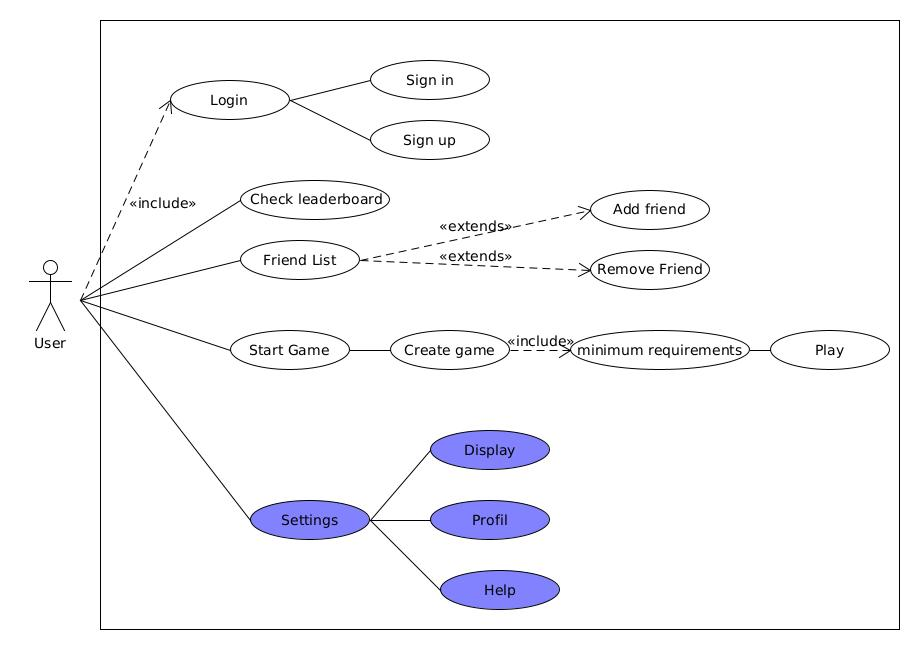
\includegraphics[width=15cm]{images/UserUseCase.jpg}
\caption{Diagramme de use case côté utilisateur}
\label{fig:UserUseCase}
\end{figure}

\subsubsection{Connexion}
En lançant le programme, l'utilisateur est invité à s'inscrire ou se connecter.

A l'inscription, un pseudonyme unique et un mot de passe lui sont demandés tant que le pseudo entré est déjà pris par quelqu'un d'autre.

Dans le cas de la connexion, on invite l'utilisateur à saisir son pseudo et son mot de passe tant que le pseudo est inexistant ou que le mot de passe ne correspond pas. Après s’être connecté, l'utilisateur accède au menu principal.

Dans les deux cas, une option de retour à la page d'accueil sera disponible.

\subsubsection{Menu principal}

- Gestion des amis:

Dans cette option, l'utilisateur peut consulter sa liste d'amis et voir le score de ces derniers. Il à la possibilité d'envoyer 
des demandes d'amitié, en accepter ou en refuser. L'utilisateur peut également supprimer des personnes de sa liste d'amis.\\

- Consulter le classement:

Le classement affiche tout les utilisateurs de l'application ainsi que leurs scores. La liste est trié du joueur ayant le plus haut score à celui avec le plus bas.  
Cette option permet au client de prendre connaissance des pseudonymes des autres pour envoyer des demandes d'amitiés.\\

- Lancer une partie:

Lorsque l'utilisateur souhaite créer une partie, il se trouve dans un lobby. Il peut y modifier les paramètres par défaut du jeu et inviter un second joueur.
La partie est lancée quand l'hôte appuie sur play.\\

- Profile:

Dans le menu profile, l'utilisateur peut consulter ses informations de compte s'il le souhaite. A savoir, son pseudo et son score.

\subsubsection{Création de partie}
La création d'une partie est une option qui envoie l'utilisateur dans un lobby permettant de modifier les paramètres du jeu.
Cette fenêtre contient déjà des paramètres par défaut.

S'il le souhaite, l'utilisateur peut modifier les options suivantes:

- Le nombre de joueurs: 

L'utilisateur a la possibilité de choisir entre un ou deux participants. Dans le cas où le nombre de participants équivaut à deux, la deuxième personne est invitée à se connecter.\\

- La difficulté de la partie:

 L'utilisateur doit choisir le niveau de difficulté  de sa partie. La difficulté de chaque niveau sera adaptée en fonction de ce choix, mais elle augmente progressivement au fur et à mesure, après chaque victoire de niveau. \\

- Le tir allié: 

La possibilité d'activer le tir allié ne peut être accordée que dans le cas où le nombre de joueurs est supérieur à un.
Le joueur aura donc le droit de choisir s'il souhaite que les projectiles de l'invité soient inoffensifs ou non et inversement. Cette option active aussi la collision entre les joueurs. \\

- Le nombre de vies: 

Le choix du nombre de vies est limité à 3 pour l'utilisateur.  Il peut donc seulement la diminuer.\\

- Bonus :
Il existe différentes sortes de bonus:
\begin{itemize}
  \item DamageUp: augmente les dégâts des projectiles
  \item Minigun: tir automatique à cadence élevée
  \item TripleShot: tir de 3 projectiles en même temps
  \item LifeSteal: chaque élimination redonne de la vie
\end{itemize}

Le joueur peut choisir la probabilité d'apparition des bonus lorsqu'il tue un ennemi. 
Ainsi il peut rendre le jeu plus ou moins difficile. 

\subsubsection{Jeu}

- Partie en cours:\\ \\
Elle reçoit les actions effectuées par les joueurs ̀à travers le serveur et les applique au jeu. 
Lors de sa création, elle possède les paramètres choisis par le joueur ainsi qu’un identifiant. 
Ce dernier permet au serveur de déterminer à quelle partie il doit envoyer l’action d’un 
utilisateur.\\

Le joueur commence chaque partie avec une à trois vies constituée(s) de 100 points de vie (sauf en cas de partie personnalisée) et
contrôle un vaisseau avec lequel il peut tirer des projectiles vers des ennemis, ce qui 
augmentera son score à chaque tir atteignant sa cible. Sa quantité de points de vie est réduite
lorsqu’il subit des dégâts. S’il n’a plus de points de vie, le joueur perd une vie. Lorsque le 
joueur n’a plus de vie, son vaisseau est détruit et si plus aucun joueur n’a de vie, la partie se 
termine. Elle peut également s’arrêter en cas de déconnexion d’un utilisateur, ou lorsque celui-ci a éliminé tous les ennemis.\\


- Niveau (par défaut):\\ \\
La partie est divisée en 4 niveaux de difficulté croissante. Au niveau 2 et 4, le(s) joueur(s) se retrouvera/ont face à un boss dont la difficulté dépendra du niveau. En passant au niveau suivant, le nombre, la santé et 
les dégâts des ennemis accroissent.\\

- Niveau (personnalisé):\\ \\
Les parties personnalisées sont constituées d'un seul niveau complètement modulable d'une durée maximum de 200 secondes. Durant cette partie, l'utilisateur fera face aux ennemis positionnés selon ses désirs et devra affronter un boss s'il en a décidé ainsi.\\ \\

- Entités à l’écran:\\ \\
Parmi les entités apparaissant à l’écran et pouvant se déplacer, il y a les vaisseaux, les bonus, 
les projectiles et les obstacles.\\ \\
\begin{itemize}
    \item[$\bullet$ Ship:]Dans ce jeu, il existe 4 types de ships : les PlayerShip, les EnemyShip (type 1 et 2) et les Boss. Tous ces vaisseaux peuvent subir et infliger des dégâts. Les PlayerShip sont les vaisseaux alliés, ce sont ceux que les joueurs contrôlent. Ils peuvent se déplacer dans toutes les directions (verticales, horizontales, diagonales).\\ Les EnemyShip peuvent lâcher un bonus en se détruisant, la probabilité de lâcher ce bonus est déterminée par l’utilisateur avant de lancer la partie. Le premier type peut uniquement se déplacer de manière verticale, alors que le second uniquement de manière horizontale.\\ Le Boss est l’ennemi final à affronter pour finir les niveaux. Le premier boss est un vaisseau beaucoup plus volumineux et résistant que les EnemyShip. Il a la capacité de se déplacer horizontalement de gauche à droite et de droite à gauche, et également de tirer 2 projectiles à la fois. Le second détient les mêmes caractéristiques, tout en ayant la capacité de tirer 4 projectiles à la fois au lieu de 2.\\ 

    \item[$\bullet$ Projectiles:]Les projectiles sont créés lorsque les vaisseaux tirent. Ils peuvent sortir de l’écran, s’annuler en rencontrant d’autres projectiles ou causer des dégâts en atteignant leur cible.\\

    \item[$\bullet$ Bonus:]Les bonus sont de plusieurs types et peuvent rapporter des améliorations d’armes et de santé au joueur qui réussit à l'attraper.
\end{itemize}
\newpage
\begin{figure}[hbtp]
\centering
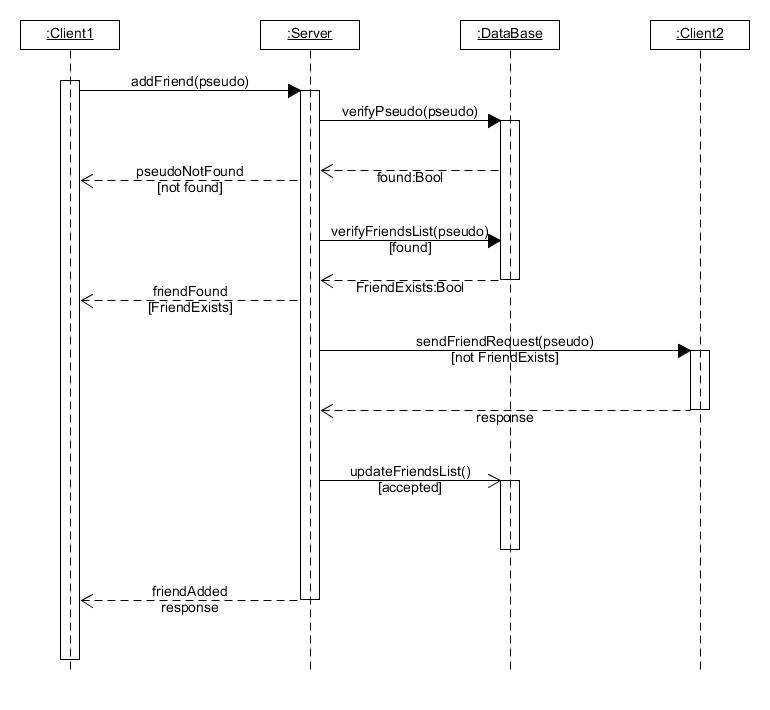
\includegraphics[scale=0.5]{images/add_friend.jpg}
\caption{Diagramme de séquence pour l'ajout d'un ami }
\end{figure}

\begin{figure}[hbtp]
\centering
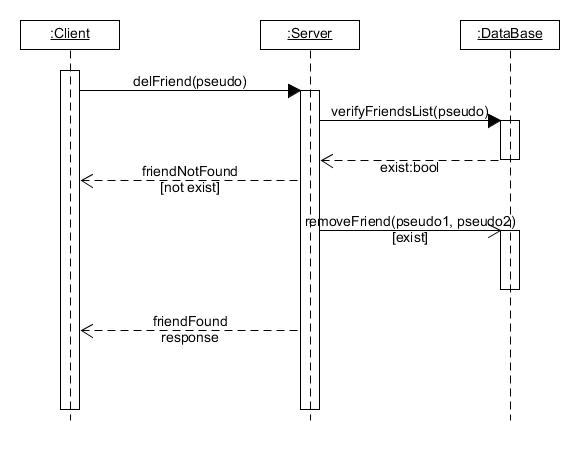
\includegraphics[scale=0.5]{images/del_friend.jpg}
\caption{Diagramme de séquence pour la suppression d'un ami }
\end{figure}


\begin{figure}[hbtp]
\centering
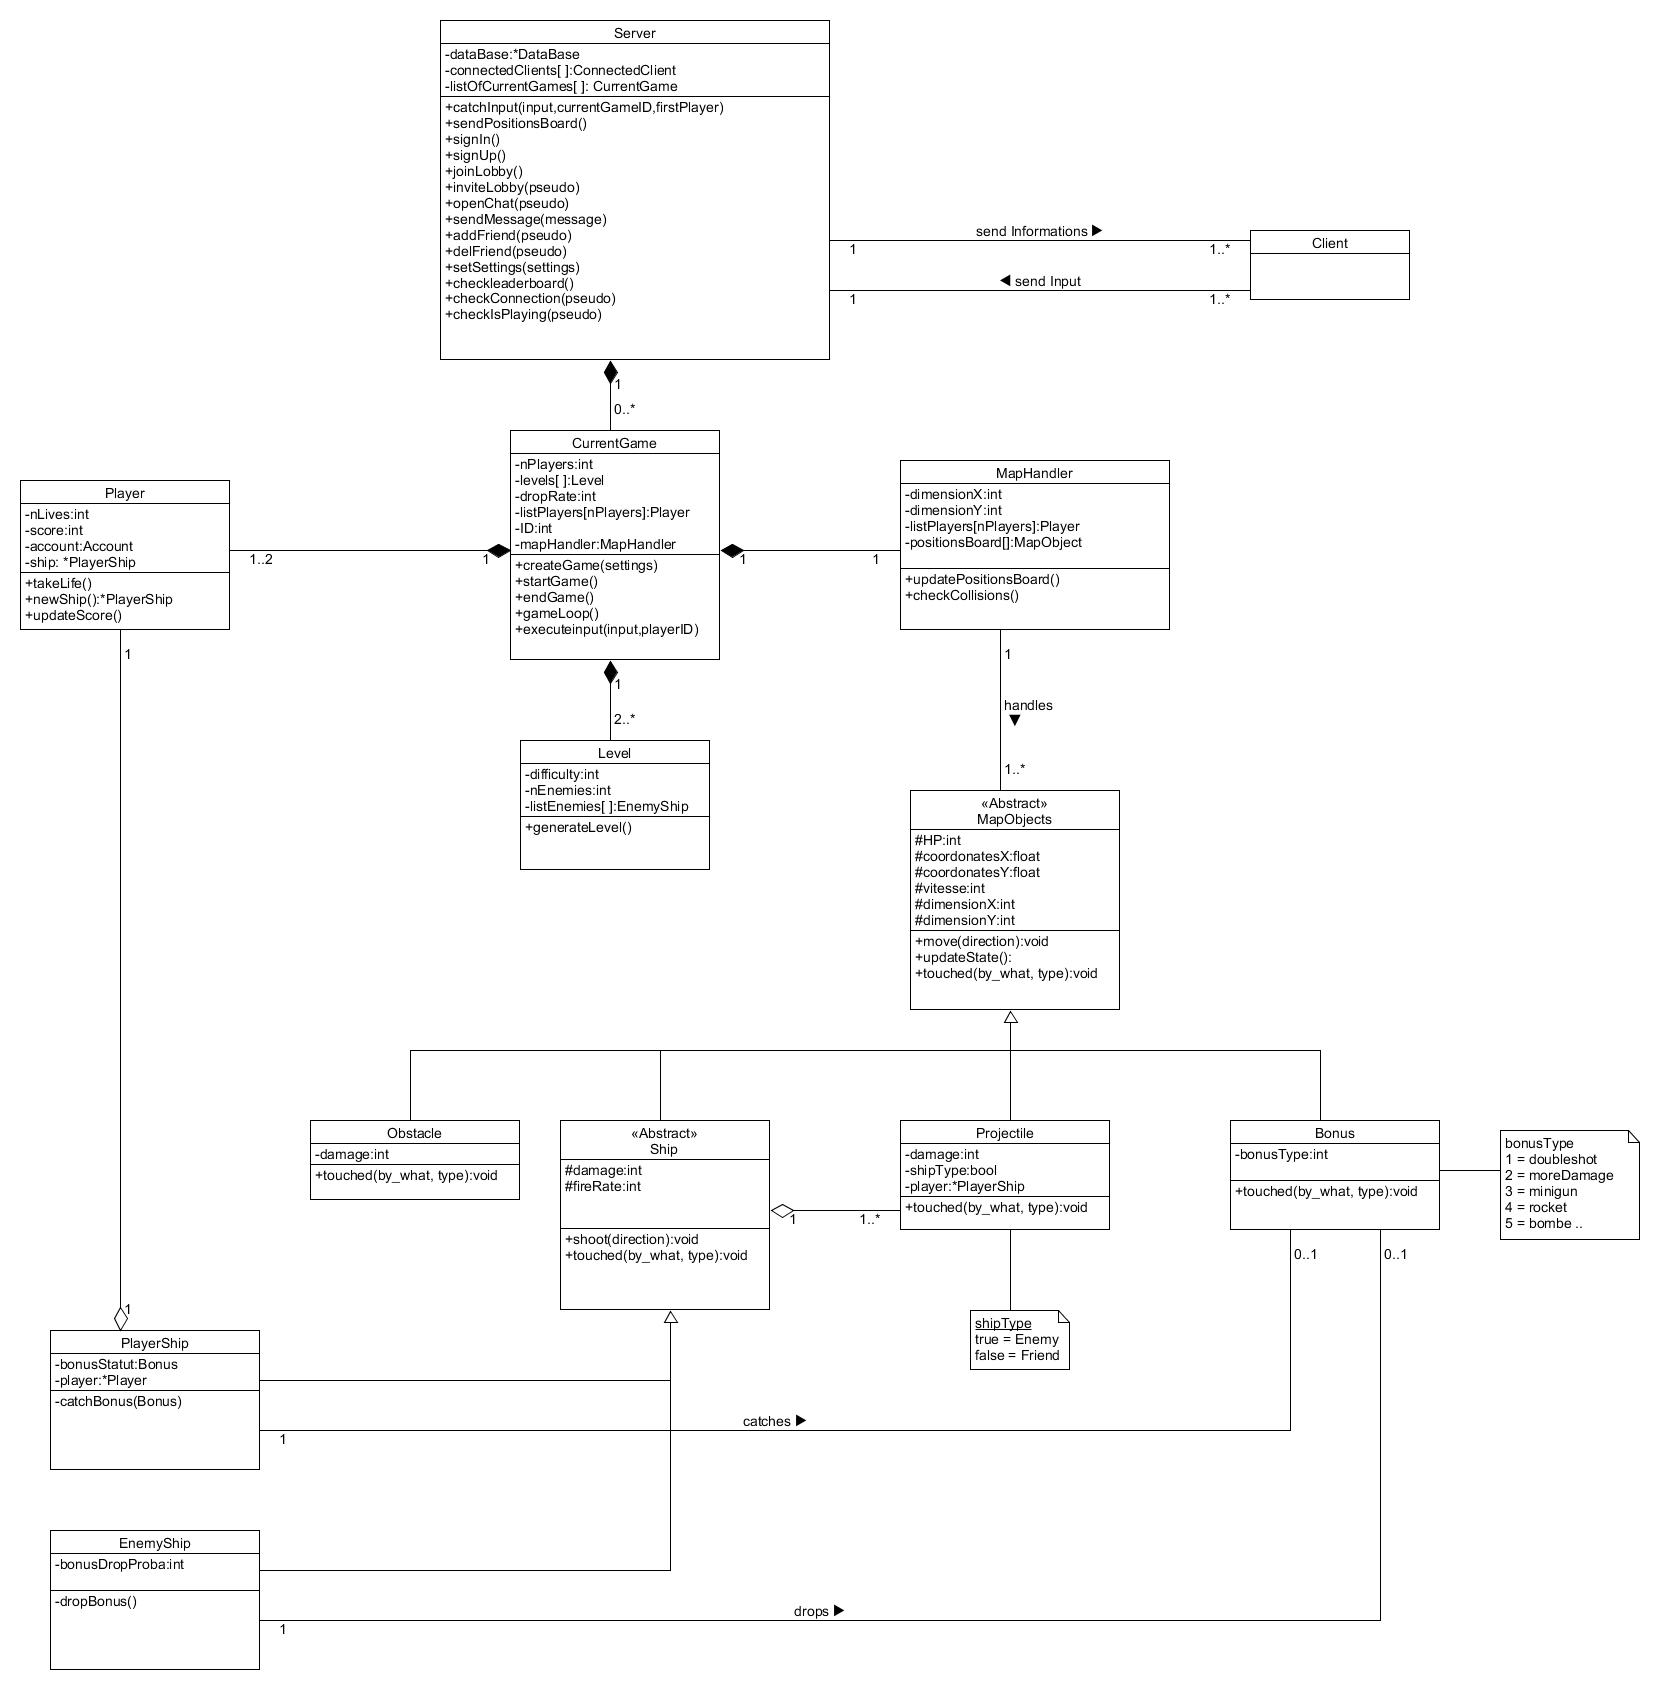
\includegraphics[scale=0.3]{images/newGameClassDiagram.jpg}
\caption{Diagramme de classe du jeu}
\end{figure}

\begin{figure}[hbtp]
\centering
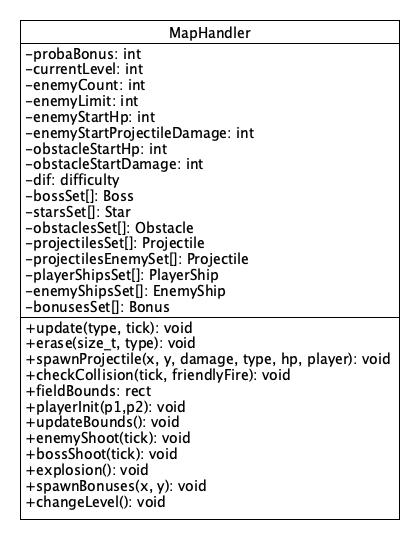
\includegraphics[scale=0.3]{images/mapHandlerDiagram.jpg}
\caption{classe MapHandler}
\end{figure}

\begin{figure}[hbtp]
\centering
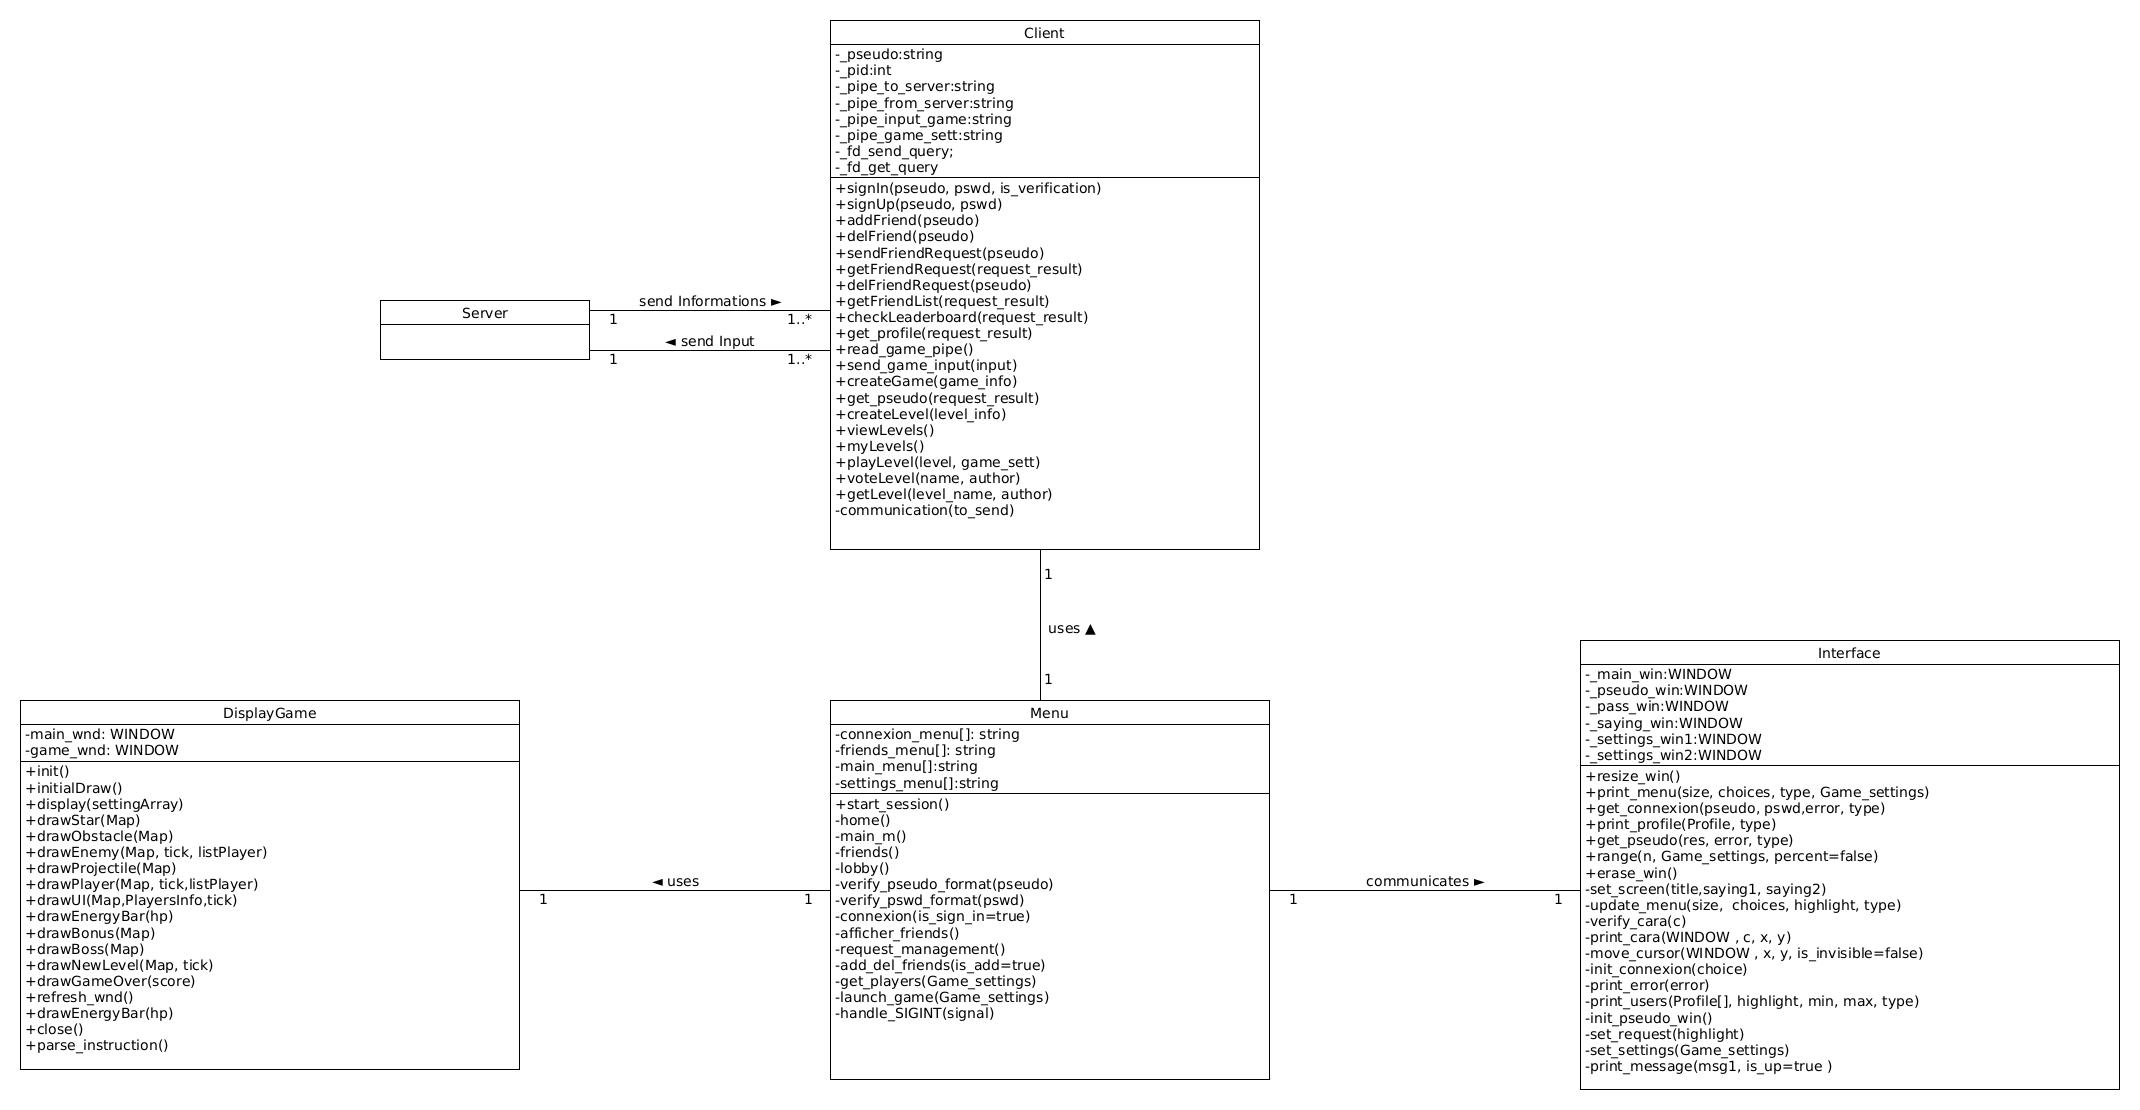
\includegraphics[scale=0.3, angle=90]{images/newClientClassDiagram.jpg}
\caption{Diagramme de classe côté client}
\end{figure}

\newpage

\section{Besoins système}
\subsection{Besoins fonctionnels}

\begin{figure}[h!]
\centering
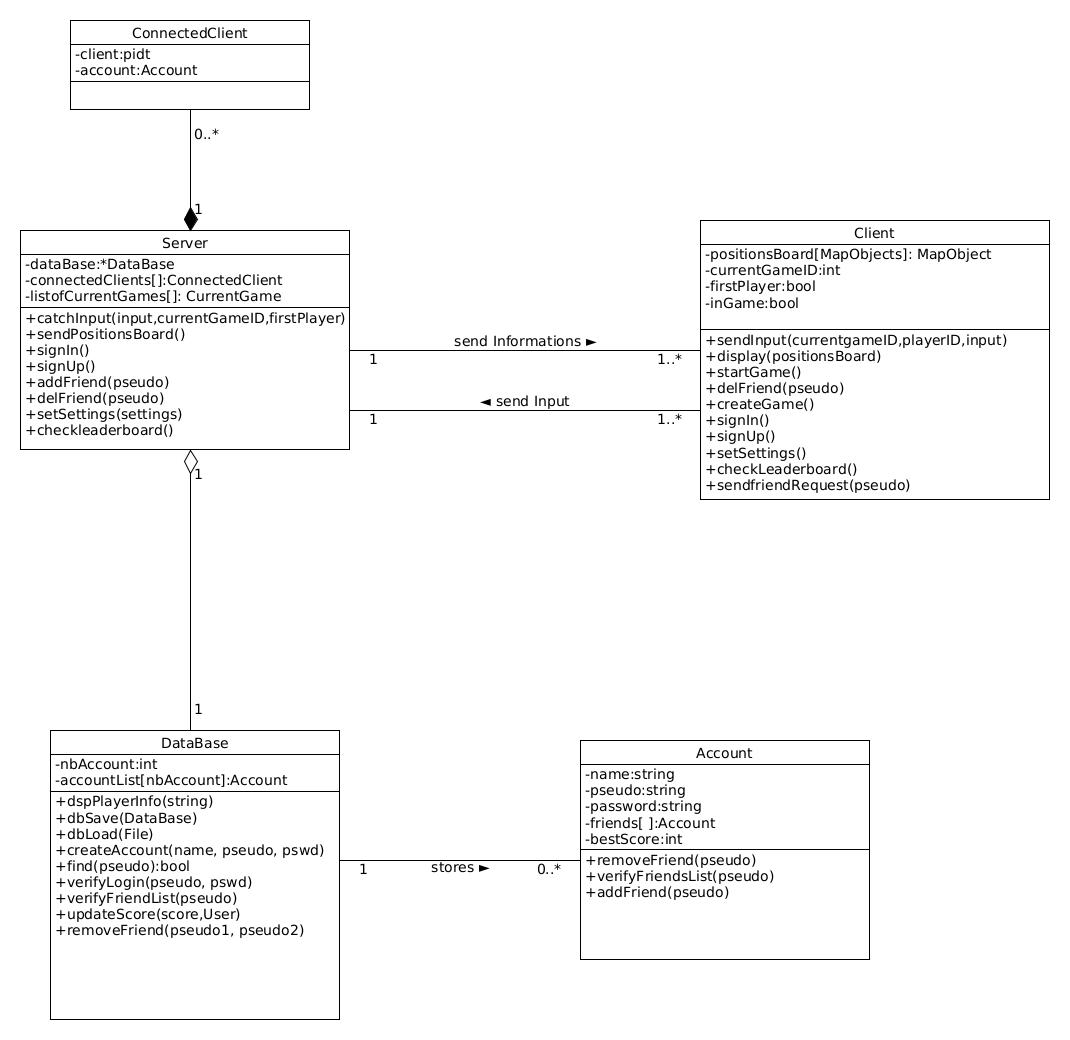
\includegraphics[width=16cm]{images/newSystemClassDiagram.jpg}
\caption{Diagramme de classe du système}
\label{fig:UerUseCase}
\end{figure}

\subsubsection{Serveur}
Le serveur est la classe principale du système. Il va gérer la majorité des interactions du programme et va servir d'intermédiaire entre le client et toutes les fonctionnalités de l'application. Pour le bon fonctionnement du programme, cette classe devra toujours être active.\\

- Communication client-serveur : \\
Le programme client et le serveur communiquent entre eux à travers des tubes de communications privés et publics. Les messages envoyés entre eux sont codifiés et limités.
Lorsqu'une session utilisateur est lancée, il notifie le serveur à travers un tube public en envoyant son identifiant (pid du processus). 
Dés lors, le serveur lui crée des tubes privées pour conserver l'intégrité des données.\\

- Connexion : \\
Lorsqu'un client souhaite se connecter ou s'inscrire, il envoie son pseudo et mot de passe au serveur. Ce dernier se charge de vérifier l'existence ou la disponibilité de ces informations dans la base de données et ainsi ouvrir une session utilisateur ou non. 

- Interactions entre utilisateurs : \\
Un client peut ajouter et supprimer des amis ainsi que voir le classement de tous les utilisateurs. 
Ces actions sont rendues possibles grâce au serveur qui sert de lien entre tous les programmes clients. 
En effet, ces derniers envoient les messages correspondants à leurs requêtes et le serveur se charge d'interroger la base de donnée et d'envoyer les réponses adéquates. \\

- Jeu : \\
Toutes les parties lancées par les utilisateurs sont gérées par le serveur. En effet, il a pour rôle de décider de toutes les actions indépendantes du client et d'appliquer les mouvements de celui-ci.
Ce qui signifie que c'est lui qui invoque les ennemis, les obstacles et les bonus. C'est aussi au serveur de recevoir les coups des joueurs, de les appliquer et de vérifier les collisions.
Dés lors, le seul rôle du programme utilisateur est d'écouter les instructions du serveur et de les appliquer. 

Une fois qu'une partie est terminée, le serveur se charge de mettre à jour le score des joueurs. Le score final est commun et est la somme des scores de chaque joueur.

- Terminaison : \\
Lorsqu'une session cliente est terminée, le serveur est mis au courant et se charge donc de supprimer les tubes de communications. S'il y a une partie en cours, elle est arrêtée. 
Dans le cas où le serveur est arrêté, tous les programmes utilisateurs ainsi que les parties lancées sont stoppées et la base de données est sauvegardée. \\

\subsubsection{DataBase}

La base de données a pour rôle de sauvegarder les informations relatives aux utilisateurs. \\
Un certains nombre d'opérations lui sont applicable à travers le serveur. En effet, ce dernier permet le transfert d'informations
entre les clients et la base de données. 
Les informations contenues dans la base de données sont les pseudonymes, mots de passe et le meilleur score de chaque compte. 

\subsubsection{Client}
La classe Client permet à l utilisateur de communiquer avec le serveur à travers diverses actions possibles affichées sur le menu.
Toutes les fonctionnalités décrites dans la section 2.1 sont possibles. A savoir : 
\begin{itemize}
    \item Se connecter
    \item S'inscrire
    \item Créer une partie
    \item Consulter le classement
    \item Gérer ses amis
    \item Consulter son profile
\end{itemize}


\subsubsection{Gestion des comptes}
Un objet Account contient toutes les informations relatives à un utilisateur (pseudo, mot de passe et score, sa liste d'amis et ses requêtes). 
Ces informations sont stockées dans la base de données et les différentes demandes d'accès à celle-ci sont traitées par le serveur.

- Accès:

Lors de la création d'un compte, la disponibilité du pseudo est vérifiée par la base de données. Si celui-ci n'est pas trouvé, un nouveau compte est bien créé et ajouté dans la base.

Lors de la connexion, c'est encore le serveur, à travers la base de données qui vérifie que le pseudo et le mot de passe saisis correspondent à un compte existant.

- Contenu d'un compte:

Chaque compte possède des informations sur l'utilisateur auquel il appartient, notamment ses identifiants (pseudo, mot de passe), son score (pour qu'il apparaisse dans le classement général des joueurs), une liste d'amis et une liste d'invitations qu'il peut consulter à tout moment.

\subsubsection{Gestion d'une partie}

Lorsque le joueur voudra lancer une partie,
il aura la possibilité de choisir les paramètres de celle-ci comme expliqué plus haut (cf 2.1.3). Si le nombre de joueurs choisi est 2, l'hôte doit obligatoirement inviter un autre utilisateur à se connecter.

La partie ne peut pas commencer tant que le second joueur ne réussit pas à se connecter.
\subsubsection{Gestion des amis}

- Ajout: Lorsque l'utilisateur veut ajouter un ami, la requête est envoyée à la base de données via le serveur. Elle effectue des vérifications et envoie la demande, si elle est valide, à la personne concernée. Si la demande est acceptée, la liste d'amis des deux utilisateurs est mise à jour.

- Suppression: La base de données fait une recherche de l'ami à supprimer et l'efface de la liste d'amis de l'utilisateur. L'utilisateur sera également supprimé de la liste de son ancien ami.

\subsubsection{Classement}

Après chaque partie, le serveur met à jour le score de chaque joueur si celui-ci est supérieur à son score actuel. 
Ce qui permet de garder le classement tous le temps à jour. 

\subsection{Besoins non fonctionnels}

- Le lancement du programme nécessite un environnement Linux possédant un dossier nommé "tmp" à la racine, afin de pouvoir stocker et supprimer les tubes créés par le serveur.\\
- Par souci de sécurité, toutes les requêtes d'un client doivent passer par le serveur.\\
- Pour des raisons esthétiques, la taille du terminal doit être de 80x24.
- La librairie open source "ncurses" est indispensable.


\\
\\\\
\begin{figure}[hbtp]
\centering
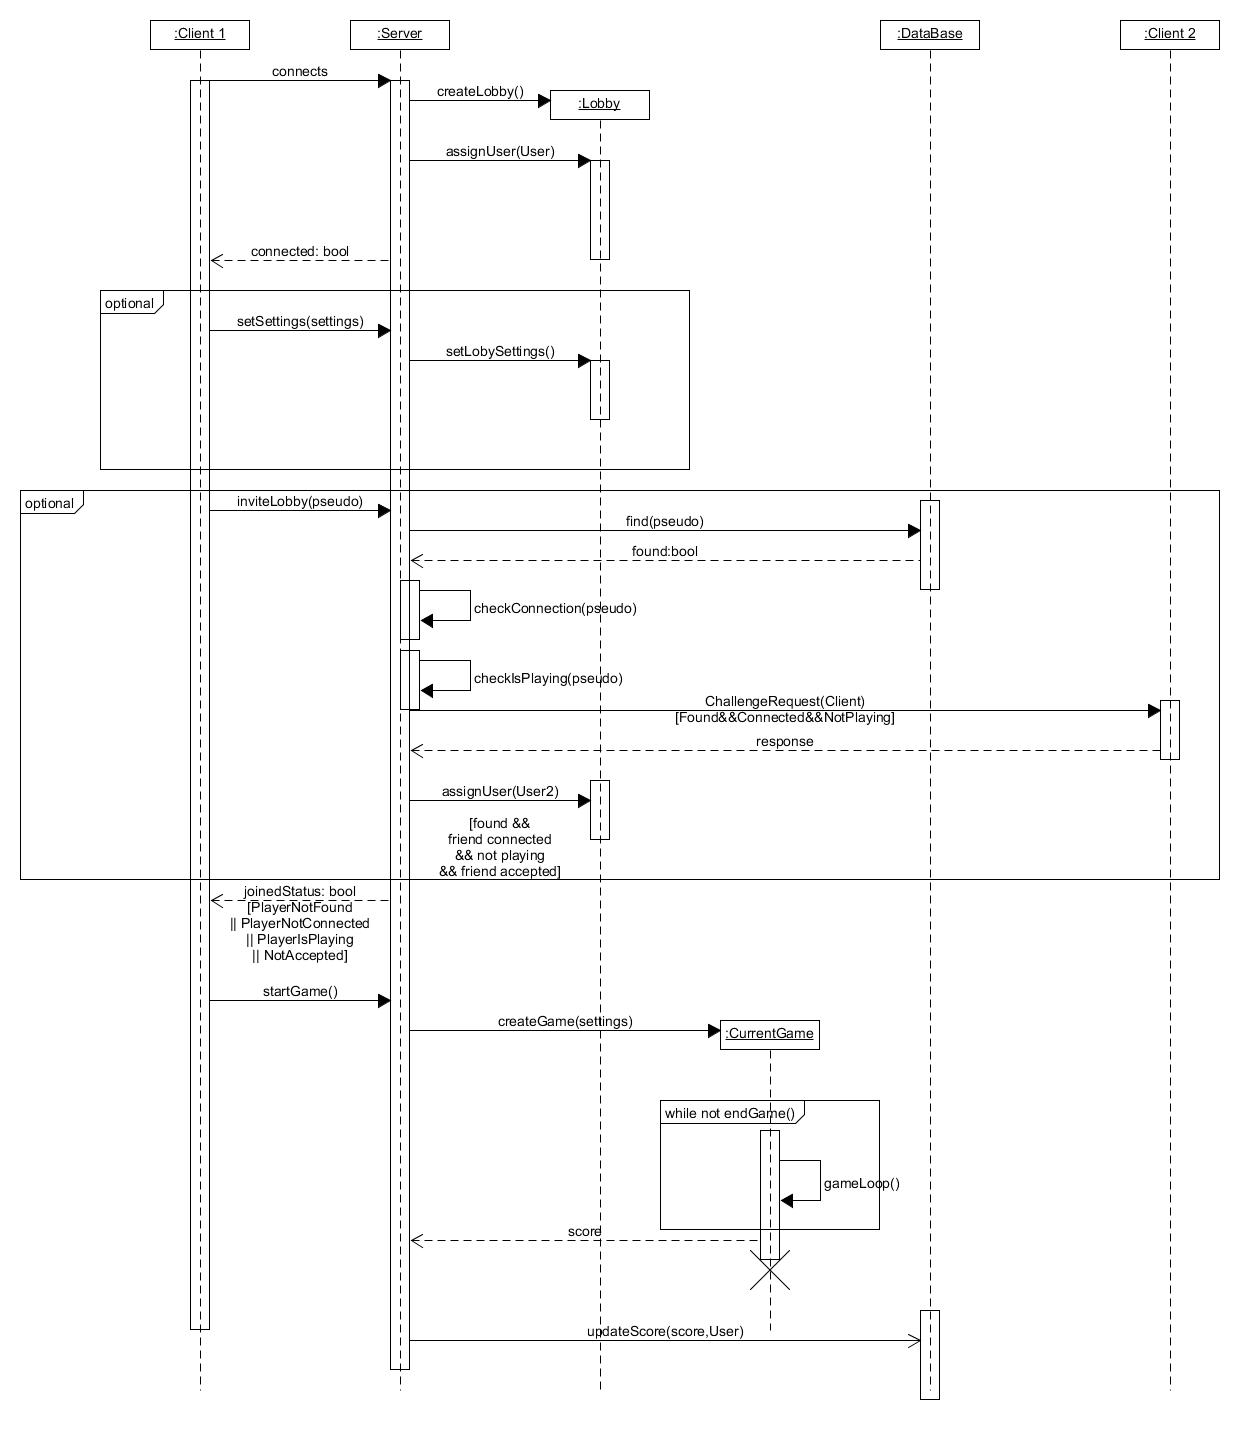
\includegraphics[scale=0.3]{images/sequence_diagram_StartGame}
\caption{Diagramme de séquence de lancement du jeu}
\end{figure}

\begin{figure}[hbtp]
\centering
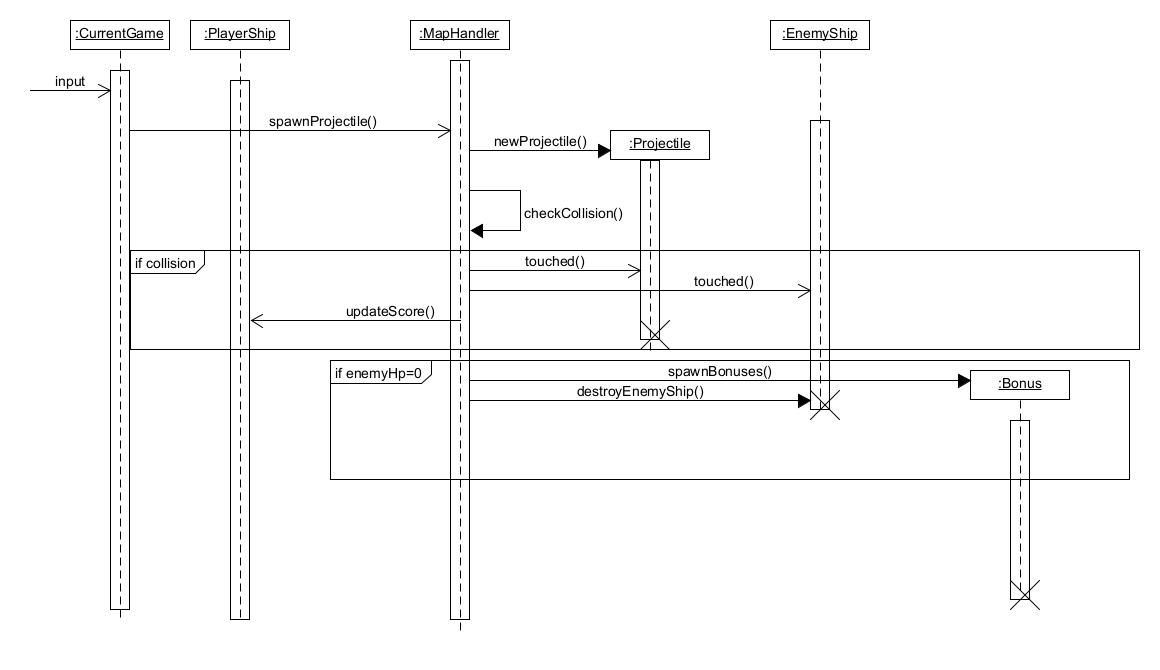
\includegraphics[scale=0.3]{images/player_shooting.jpg}
\caption{Diagramme de séquence d'un tir de joueur}
\end{figure}


\begin{figure}[hbtp]
\centering
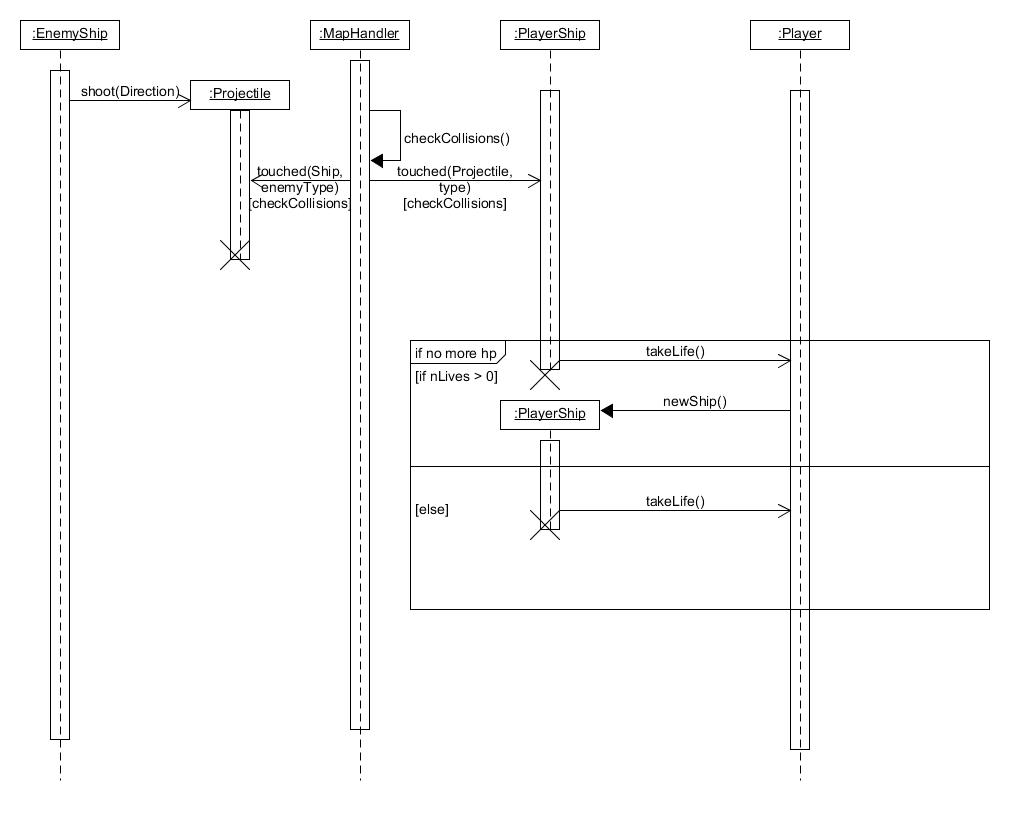
\includegraphics[scale=0.3]{images/enemy_shooting.jpg}
\caption{Diagramme de séquence d'un tir ennemi }
\end{figure}

\newpage
\section{Annexes}
\subsection{ Description du diagramme use case utilisateur}

\begin{center}
\begin{longtable}{|p{1,5cm}||p{3,5cm}|p{3,5cm}|p{3,5cm}|p{3,5cm}|}
\hline
\rowcolor{green}
USE CASE   &\center{Pré-conditions}   & \hfill Post-conditions \hfill\null & Cas Général & Cas exceptionnels\\
\hline
\hline
\textbf{Sign in}      & L'utilisateur doit être enregistré dans la base de données  & L'utilisateur est connecté à sa base de données et le menu principal est affiché & L'utilisateur déjà enregistré se connecte à son compte en entrant son pseudonyme et mot de passe. Le serveur vérifie que les données soient correctes et donne accès au compte du client  & Si l’identifiant ou le mot de passe sont incorrects, affiche un message d'erreur est affiché à l'utilisateur \\
\hline
\hline
\textbf{Sign up}     & L'utilisateur n'est pas présent dans la base de données   & Ajout d'un compte dans la base de données et affichage du menu principal & L'utilisateur crée un compte en introduisant un pseudo et un mot de passe  & Si les données entrées ne respectent pas le format requis ou que le pseudonyme est déjà utilisé, un message d'erreur est affiché et l'utilisateur peut recommencer l'action jusqu'à ce qu'elle soit valide \\

\hline
\hline
\textbf{Create game}    & L'utilisateur doit être enregistré dans la base de données  & Possibilité de sauvegarder les paramètres par défaut d'une partie  & L'utilisateur peut lancer une partie après avoir rempli les conditions minimales  & Néant \\
\hline
\hline
\textbf{Check Leaderboard}  & L'utilisateur doit être enregistré dans la base de données   & \hfill Néant  \hfill\null &Le joueur peut consulter le classement des scores en envoyant une requête au serveur qui va lui renvoyer les informations  & Néant \\
\hline
\hline
\textbf{View friend list }   & L'utilisateur doit être enregistré dans la base de données   & Néant  & Consultation de liste d'ami dans la base de données & Néant \\
\hline
\hline
\textbf{Add friend}    & L'utilisateur doit être enregistré dans la base de données   & Si invitation acceptée, ajout d'amis dans la base de donnée (bidirectionnel) & Entrer le pseudo d’un utilisateur. Le système va rechercher dans la base de données si le pseudo existe et lui envoyer une invitation.  & Ajouter un pseudo qui n’existe pas (affiche une erreur)\\
\hline
\hline
\textbf{Delete friend}    & L'utilisateur doit être enregistré dans la base de données et avoir au moins un ami.   & Suppression dans la liste d’amis par le serveur(bidirectionnel)  & Entrer le pseudo d’un ami. Le serveur va rechercher dans la base de données si le pseudo existe et le supprimer.  & Supprimer un ami qui n’existe pas (affiche une erreur) \\
\hline
\hline
\textbf{Profile}     & L'utilisateur doit être enregistré dans la base de données   & Mise à jour des changements  & L'utilisateur peut consulter ses informations de profile. Neant  & Néant\\
\hline
\hline
\textbf{Ship’s controls}  & Créer une partie  & Actualisation de l’état de jeu  & Se déplacer, tirer recevoir des bonus  & Néant\\
\hline
\textbf{Leave party}      & Être en train de jouer   & Retour au menu principal  & Le joueur arrête la partie en cours.  & Néant\\
\hline
\hline
\hline
\hline
\textbf{Leave game}      & Etre connecté   & Fermeture du jeu  & L'utilisateur est connecté et veut quitter le jeu  & L'utilisateur est connecté et force sa sortie du jeu (CTRL+C, ...)\\
\hline
\end{longtable}
\end{center}


\end{document}
